\documentclass[a4paper, 12pt]{article}
\usepackage{physics, amsmath, amsfonts, fixmath, geometry, tikz, pgf, multirow, hyperref, amsfonts,amssymb, mathtools, physics, xcolor, siunitx, subcaption,tcolorbox}


\pdfpagewidth 8.5in
\pdfpageheight 11in
\headheight 0pt
\headsep 0pt
\footskip .25in
\marginparwidth 0pt
\marginparsep 0pt
\oddsidemargin \dimexpr 1in -1in
\topmargin \dimexpr 1in -1in
\textwidth \dimexpr \pdfpagewidth -2\oddsidemargin -2in
\textheight \dimexpr \pdfpageheight -2\topmargin -2in
%Commands

\newtcolorbox{boxes}[3][]
{
	colframe = #2!25,
	colback  = #2!10,
	coltitle = #2!40!black,  
	title    = {\textbf{#3}},
	#1,
}
\usepackage{graphicx}
\usepackage{xepersian}
\usepackage{braket}
\settextfont[]{XB Niloofar}
\title{\textbf{
جدول ضرب گروه 
$D_5$
}}
\author{مربوط به تمرین اول - سوال پنجم}
\date{}

\begin{document}
\maketitle
جدول ضرب گروه را چطور بسازیم؟
در این نوشته من فقط دوتا از اعضای جدول ضرب گروه 
$D_5$
رو براتون به شکل صریح می‌نویسم؛ شما با خواندنش می‌تونید کامل جدول رو پر کنید.

\vspace{1em}
\noindent
با نحوه عمل اعضای گروه 
$D_5$
روی پنج‌ضلعی منتظم که آشنا هستید. (اشکال
\ref{ac1}
و
\ref{ac2}
و 
\ref{ac3}
)

\begin{figure}[h]
	\centering
	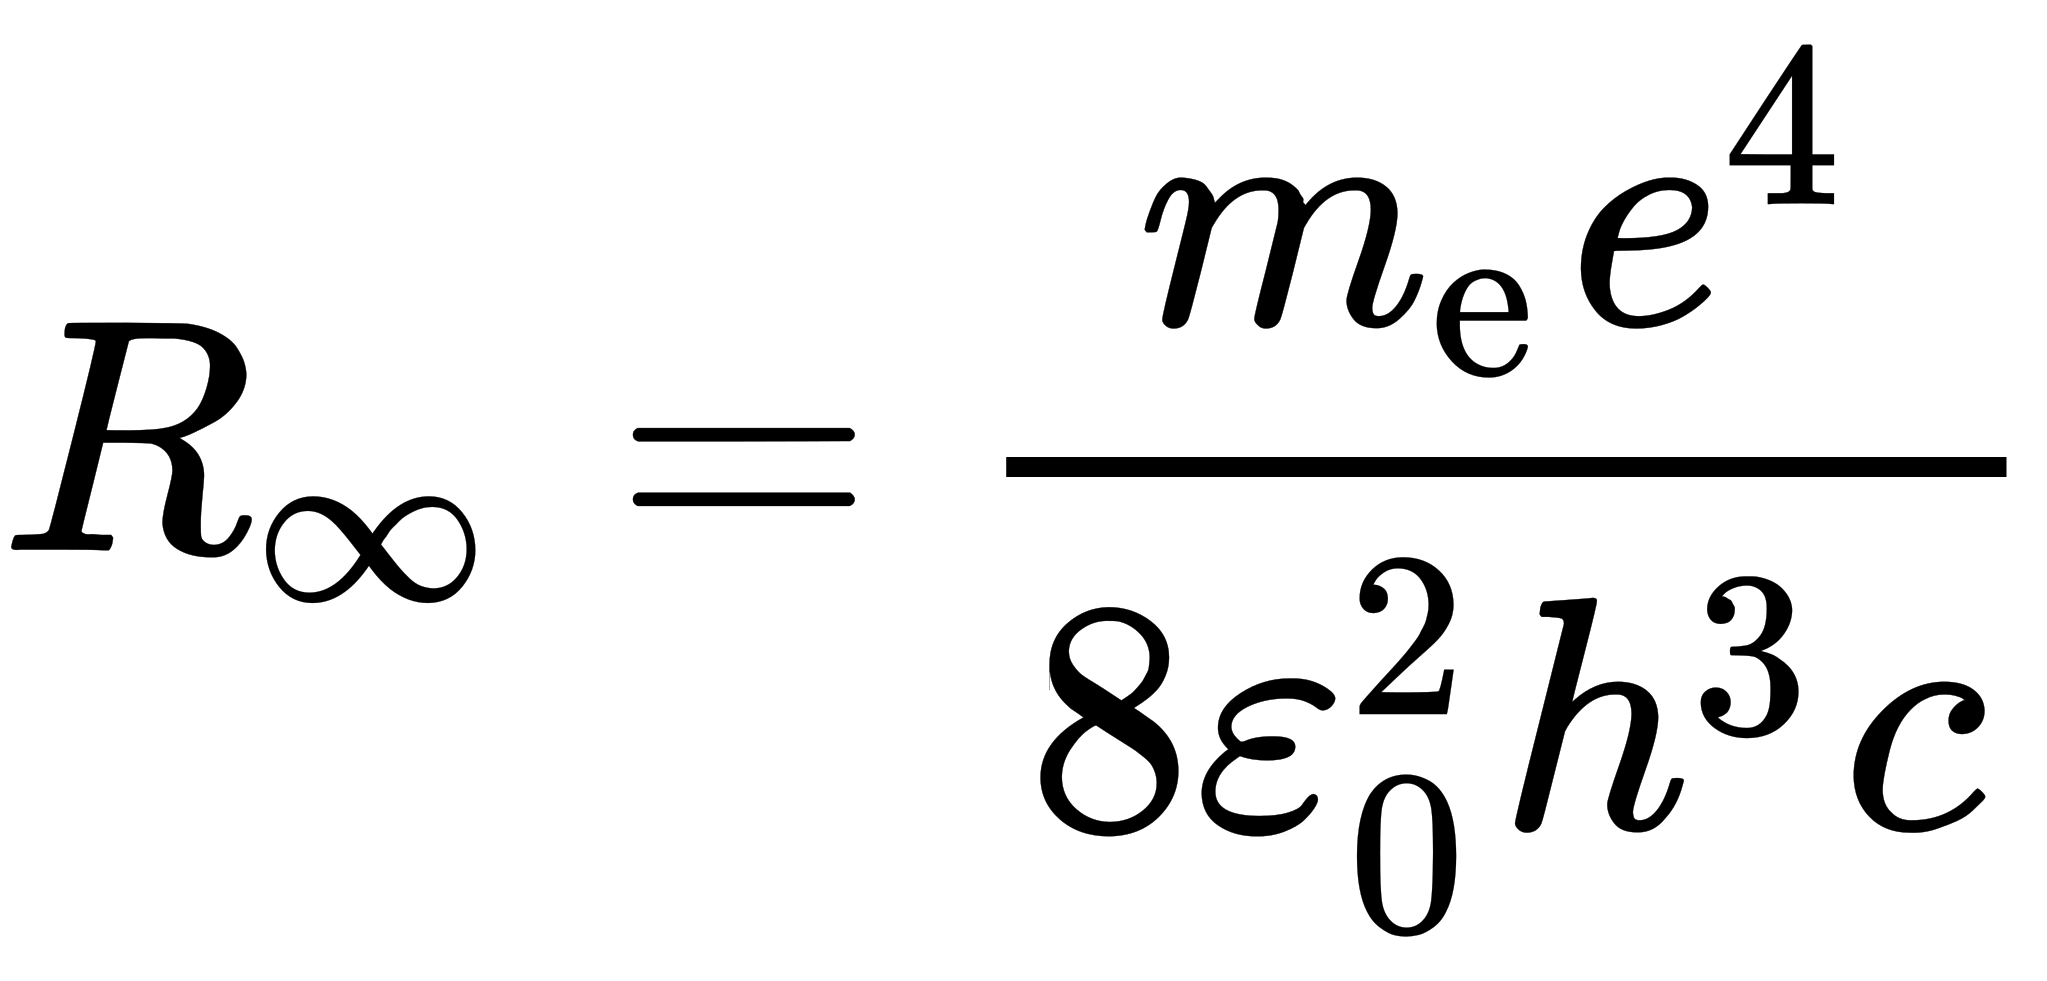
\includegraphics[width=28em]{1.png}
	\caption{اثر دو عضو از گروه
	$D_5$
	روی پنج ضلعی منتظم. }
	\label{ac1}
\end{figure}
\begin{figure}[h]
	\centering
	\includegraphics[width=10em]{2.png}
	\caption{زاویه چرخش دوران‌ها }
	\label{ac2}
\end{figure}
\begin{figure}[h]
	\centering
	\includegraphics[width=15em]{3.png}
	\caption{محور بازتاب اعضای
	$T_i$. }
	\label{ac3}
\end{figure}
حالا جدول ضرب گروه را (شکل
\ref{prodtab}
) در نظر بگیرید:
\begin{figure}[h]
	\centering
	\includegraphics[width=25em]{4.png}
	\caption{جدول ضرب گروه 
	$D_5$.
	 }
	 \label{prodtab}
\end{figure}

\noindent
می‌خواهیم دو خانه‌ی قرمز و سبز رنگ شکل
\ref{prodtab}
را پر کنیم.

\noindent
 خانه‌ی قرمز رنگ معنایش این است که اگر اول عمل 
$T_1$
و سپس عمل 
$R_1$
را انجام دهیم؛ حاصل آن مثل کدام یک از اعضای گروه است؟ شکل 
\ref{firstex}
را ببنید:
\begin{figure}[h]
	\centering
	\includegraphics[width=35em]{5.png}
	\caption{عمل متوالی: اول 
	$T_1$ و بعد 
	$R_1$
.
	}
	\label{firstex}
\end{figure}
این دقیقا مثلا 
$T_4$
اثر می‌کند( شکل 
\ref{firstex2}
)

\begin{figure}[h]
	\centering
	\includegraphics[width=25em]{6.png}
	\caption{اثر
		 $T_4$.
	}
	\label{firstex2}
\end{figure}



\vspace{1em}
\noindent
معنای خانه‌ی سبز رنگ این است که اول
$T_2$ و سپس 
$T_3$
اثر کند. در شکل
\ref{secondex}
این عمل را می‌بینید.
\begin{figure}[h]
	\centering
	\includegraphics[width=35em]{7.png}
	\caption{عمل متوالی: اول 
		$T_2$ و بعد 
		$T_3$
		.
	}
	\label{secondex}
\end{figure}

\noindent
این عمل ترکیبی مشابه 
$R_2$
است؛ همانطور که در شکل 
\ref{secondex2}
می‌بینید.

\begin{figure}[h]
	\centering
	\includegraphics[width=25em]{8.png}
	\caption{عمل
		$R_2$
		.
	}
	\label{secondex2}
\end{figure}

\vspace{0.5em}
\noindent
پس دو خانه‌ی مذکور از جدول‌ضرب مشابه شکل 
\ref{prodtabsemi}
تکمیل می‌شوند.
\begin{figure}[h]
	\centering
	\includegraphics[width=25em]{9.png}
	\caption{جدول‌ضرب پس از تکمیل دوخانه‌ی سبز و قرمز	.
	}
	\label{prodtabsemi}
\end{figure}









\end{document}